\documentclass[11pt]{article}\usepackage[]{graphicx}\usepackage[]{color}
% maxwidth is the original width if it is less than linewidth
% otherwise use linewidth (to make sure the graphics do not exceed the margin)
\makeatletter
\def\maxwidth{ %
  \ifdim\Gin@nat@width>\linewidth
    \linewidth
  \else
    \Gin@nat@width
  \fi
}
\makeatother

\definecolor{fgcolor}{rgb}{0.345, 0.345, 0.345}
\newcommand{\hlnum}[1]{\textcolor[rgb]{0.686,0.059,0.569}{#1}}%
\newcommand{\hlstr}[1]{\textcolor[rgb]{0.192,0.494,0.8}{#1}}%
\newcommand{\hlcom}[1]{\textcolor[rgb]{0.678,0.584,0.686}{\textit{#1}}}%
\newcommand{\hlopt}[1]{\textcolor[rgb]{0,0,0}{#1}}%
\newcommand{\hlstd}[1]{\textcolor[rgb]{0.345,0.345,0.345}{#1}}%
\newcommand{\hlkwa}[1]{\textcolor[rgb]{0.161,0.373,0.58}{\textbf{#1}}}%
\newcommand{\hlkwb}[1]{\textcolor[rgb]{0.69,0.353,0.396}{#1}}%
\newcommand{\hlkwc}[1]{\textcolor[rgb]{0.333,0.667,0.333}{#1}}%
\newcommand{\hlkwd}[1]{\textcolor[rgb]{0.737,0.353,0.396}{\textbf{#1}}}%
\let\hlipl\hlkwb

\usepackage{framed}
\makeatletter
\newenvironment{kframe}{%
 \def\at@end@of@kframe{}%
 \ifinner\ifhmode%
  \def\at@end@of@kframe{\end{minipage}}%
  \begin{minipage}{\columnwidth}%
 \fi\fi%
 \def\FrameCommand##1{\hskip\@totalleftmargin \hskip-\fboxsep
 \colorbox{shadecolor}{##1}\hskip-\fboxsep
     % There is no \\@totalrightmargin, so:
     \hskip-\linewidth \hskip-\@totalleftmargin \hskip\columnwidth}%
 \MakeFramed {\advance\hsize-\width
   \@totalleftmargin\z@ \linewidth\hsize
   \@setminipage}}%
 {\par\unskip\endMakeFramed%
 \at@end@of@kframe}
\makeatother

\definecolor{shadecolor}{rgb}{.97, .97, .97}
\definecolor{messagecolor}{rgb}{0, 0, 0}
\definecolor{warningcolor}{rgb}{1, 0, 1}
\definecolor{errorcolor}{rgb}{1, 0, 0}
\newenvironment{knitrout}{}{} % an empty environment to be redefined in TeX

\usepackage{alltt}
\usepackage{amsmath}
\usepackage{amssymb}
\usepackage{geometry}
\usepackage{graphicx}
\usepackage{url}
\usepackage{fullpage}
\IfFileExists{upquote.sty}{\usepackage{upquote}}{}
\begin{document}
\setlength\parindent{0pt}

\Large
\textbf{Lab 2: Subsetting and Basic Data Summaries}\\
\large
\textbf{STAT 630, Fall 2021}\\
\normalsize

Remark:  This lab borrows from the ``Introduction to Data" lab available here:\\ \url{https://m.openintro.org/stat/labs.php}.    


\section{BRFSS Data Set}

The Behavioral Risk Factor Surveillance System (BRFSS) is an annual telephone 
survey of over 400,000 people in the United States. The survey is conducted by the Centers for Disease Control and Prevention (CDC), a government agency focused on public health issues.  As its name implies, the BRFSS 
is designed to identify risk factors in the adult population and report 
emerging health trends. For example, respondents are asked about their diet and 
weekly physical activity, their HIV/AIDS status, possible tobacco use, and level of healthcare coverage. The BRFSS web site 
\url{http://www.cdc.gov/brfss} contains a complete 
description of the survey, including the research questions that motivate the 
study and many interesting results derived from the data.\\

We will focus on a random sample of 20,000 people from the BRFSS survey 
conducted in the year 2000. While there are over 200  variables in this data set, we will
work with a small subset.\\

Run the following command to load the data set of 20,000 observations into your R workspace. 

\begin{knitrout}
\definecolor{shadecolor}{rgb}{0.969, 0.969, 0.969}\color{fgcolor}\begin{kframe}
\begin{alltt}
\hlstd{cdc} \hlkwb{<-} \hlkwd{readRDS}\hlstd{(}\hlkwd{url}\hlstd{(}\hlstr{"https://ericwfox.github.io/data/cdc.rds"}\hlstd{))}
\end{alltt}
\end{kframe}
\end{knitrout}


To view the variable names and dimension of the \texttt{cdc} data frame type the following commands.

\begin{knitrout}
\definecolor{shadecolor}{rgb}{0.969, 0.969, 0.969}\color{fgcolor}\begin{kframe}
\begin{alltt}
\hlkwd{names}\hlstd{(cdc)}
\end{alltt}
\begin{verbatim}
## [1] "genhlth"  "exerany"  "hlthplan" "smoke100" "height"   "weight"   "wtdesire"
## [8] "age"      "gender"
\end{verbatim}
\begin{alltt}
\hlkwd{dim}\hlstd{(cdc)}
\end{alltt}
\begin{verbatim}
## [1] 20000     9
\end{verbatim}
\end{kframe}
\end{knitrout}

We can see clearly now the the data frame contains 20,000 entries (rows) on 9 variables.  Each of the variables 
corresponds to a question that was asked in the survey.  Descriptions of the variables are provided below:  
\begin{itemize}
\item \texttt{genhlth}: a categorical variable indicating general health, with categories excellent, very good, good, fair, and poor
\item \texttt{exerany}: a categorical variable, 1 if the respondent exercised in the past month and 0 otherwise
\item \texttt{hlthplan}: a categorical variable, 1 if the respondent has some form of health coverage and 0 otherwise
\item \texttt{smoke100}: a categorical variable, 1 if the respondent has smoked at least 100 cigarettes in their entire life and 0 otherwise
\item \texttt{height}: a numerical variable, respondent's height in inches
\item \texttt{weight}: a numerical variable, respondent's weight in pounds
\item \texttt{wtdesire}: a numerical variable, respondent's desired weight in pounds
\item \texttt{age}: a numerical variable, respondent's age in years
\item \texttt{gender}: a categorical variable, respondent's gender\\
\end{itemize}

\normalsize
We can have a look at the first several rows of the data with the command

\begin{knitrout}
\definecolor{shadecolor}{rgb}{0.969, 0.969, 0.969}\color{fgcolor}\begin{kframe}
\begin{alltt}
\hlkwd{head}\hlstd{(cdc)}
\end{alltt}
\begin{verbatim}
##     genhlth exerany hlthplan smoke100 height weight wtdesire age gender
## 1      good       0        1        0     70    175      175  77      m
## 2      good       0        1        1     64    125      115  33      f
## 3      good       1        1        1     60    105      105  49      f
## 4      good       1        1        0     66    132      124  42      f
## 5 very good       0        1        0     61    150      130  55      f
## 6 very good       1        1        0     64    114      114  55      f
\end{verbatim}
\end{kframe}
\end{knitrout}

You could also look at all of the data frame at once by typing its name into 
the console, but that might be unwise here.  We know \texttt{cdc} has 20,000 rows, so 
viewing the entire data set would mean flooding your screen.  It's better to 
take small peeks at the data with \texttt{head()}, \texttt{tail()} or the indexing techniques covered during the last lab.
\clearpage

\section{Summaries and Tables}

The BRFSS questionnaire is a massive trove of information.  A good first step in
any analysis is to distill all of that information into a few summary statistics
and graphics.  As a simple example, the function \texttt{summary()} returns a numerical 
summary: minimum, first quartile, median, mean, third quartile, and maximum. 
For \texttt{weight} this is

\begin{knitrout}
\definecolor{shadecolor}{rgb}{0.969, 0.969, 0.969}\color{fgcolor}\begin{kframe}
\begin{alltt}
\hlkwd{summary}\hlstd{(cdc}\hlopt{$}\hlstd{weight)}
\end{alltt}
\begin{verbatim}
##    Min. 1st Qu.  Median    Mean 3rd Qu.    Max. 
##    68.0   140.0   165.0   169.7   190.0   500.0
\end{verbatim}
\end{kframe}
\end{knitrout}

As discussed in the previous lab, R also has built-in functions to compute summary statistics one at a time.  For example:

\begin{knitrout}
\definecolor{shadecolor}{rgb}{0.969, 0.969, 0.969}\color{fgcolor}\begin{kframe}
\begin{alltt}
\hlkwd{mean}\hlstd{(cdc}\hlopt{$}\hlstd{weight)}
\end{alltt}
\begin{verbatim}
## [1] 169.683
\end{verbatim}
\begin{alltt}
\hlkwd{median}\hlstd{(cdc}\hlopt{$}\hlstd{weight)}
\end{alltt}
\begin{verbatim}
## [1] 165
\end{verbatim}
\begin{alltt}
\hlkwd{sd}\hlstd{(cdc}\hlopt{$}\hlstd{weight)}
\end{alltt}
\begin{verbatim}
## [1] 40.08097
\end{verbatim}
\end{kframe}
\end{knitrout}

While it makes sense to describe a numerical variable like \texttt{weight} in terms
of these statistics, what about categorical data?  We could instead consider the frequency or relative frequency distribution.  The function \texttt{table()} does
this for you by counting the number of times each kind of response was given.
For example, to see the number of people who have smoked 100 cigarettes in their
lifetime, type

\begin{knitrout}
\definecolor{shadecolor}{rgb}{0.969, 0.969, 0.969}\color{fgcolor}\begin{kframe}
\begin{alltt}
\hlkwd{table}\hlstd{(cdc}\hlopt{$}\hlstd{smoke100)}
\end{alltt}
\begin{verbatim}
## 
##     0     1 
## 10559  9441
\end{verbatim}
\end{kframe}
\end{knitrout}

or instead look at the relative frequency distribution by typing

\begin{knitrout}
\definecolor{shadecolor}{rgb}{0.969, 0.969, 0.969}\color{fgcolor}\begin{kframe}
\begin{alltt}
\hlkwd{table}\hlstd{(cdc}\hlopt{$}\hlstd{smoke100)}\hlopt{/}\hlnum{20000}
\end{alltt}
\begin{verbatim}
## 
##       0       1 
## 0.52795 0.47205
\end{verbatim}
\end{kframe}
\end{knitrout}

Next, we make a bar plot of the entries in the table by putting the table inside the 
\texttt{barplot()} command.

\begin{knitrout}
\definecolor{shadecolor}{rgb}{0.969, 0.969, 0.969}\color{fgcolor}\begin{kframe}
\begin{alltt}
\hlkwd{barplot}\hlstd{(}\hlkwd{table}\hlstd{(cdc}\hlopt{$}\hlstd{smoke100))}
\end{alltt}
\end{kframe}
\end{knitrout}
\begin{knitrout}
\definecolor{shadecolor}{rgb}{0.969, 0.969, 0.969}\color{fgcolor}
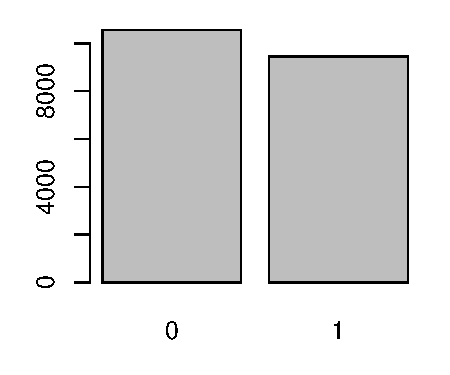
\includegraphics[width=\maxwidth]{figure/unnamed-chunk-10-1} 
\end{knitrout}

Notice what we've done here! We've computed the table of \texttt{cdc\$smoke100} and then
immediately applied the graphical function, \texttt{barplot()}. This is an important 
idea: R commands can be nested. You could also break this into two steps by 
typing the following:

\begin{knitrout}
\definecolor{shadecolor}{rgb}{0.969, 0.969, 0.969}\color{fgcolor}\begin{kframe}
\begin{alltt}
\hlstd{smoke_tb} \hlkwb{<-} \hlkwd{table}\hlstd{(cdc}\hlopt{$}\hlstd{smoke100)}
\hlkwd{barplot}\hlstd{(smoke)}
\end{alltt}
\end{kframe}
\end{knitrout}

The \texttt{table()} command can be used to tabulate any number of variables that you 
provide.  For example, to examine which participants have smoked across each 
gender, we could use the following.

\begin{knitrout}
\definecolor{shadecolor}{rgb}{0.969, 0.969, 0.969}\color{fgcolor}\begin{kframe}
\begin{alltt}
\hlkwd{table}\hlstd{(cdc}\hlopt{$}\hlstd{gender,cdc}\hlopt{$}\hlstd{smoke100)}
\end{alltt}
\begin{verbatim}
##    
##        0    1
##   f 6012 4419
##   m 4547 5022
\end{verbatim}
\end{kframe}
\end{knitrout}

Here, we see column labels of 0 and 1. Recall that 1 indicates a respondent has
smoked at least 100 cigarettes. The rows refer to gender. To include the row and column totals use \texttt{addmargins()}.

\begin{knitrout}
\definecolor{shadecolor}{rgb}{0.969, 0.969, 0.969}\color{fgcolor}\begin{kframe}
\begin{alltt}
\hlkwd{addmargins}\hlstd{(}\hlkwd{table}\hlstd{(cdc}\hlopt{$}\hlstd{gender, cdc}\hlopt{$}\hlstd{smoke100))}
\end{alltt}
\begin{verbatim}
##      
##           0     1   Sum
##   f    6012  4419 10431
##   m    4547  5022  9569
##   Sum 10559  9441 20000
\end{verbatim}
\end{kframe}
\end{knitrout}

\section{Subsetting Data Frames}

The first lab went over how to extract rows, columns, and specific elements of a data frame using indexing (i.e., brackets \texttt{[]}) or by using \texttt{\$} to extract columns (variables) by their names.  However, it is also useful to extract rows of a data frame that have specific characteristics.  For instance, suppose we want the extract the rows of the \texttt{cdc} data frame that correspond to a certain gender (male or female), or extract the rows corresponding to respondents who are over 40 years old.  To do this we can use logical expressions and subsetting techniques.\\

To illustrate logical operations in R, lets work with a smaller portion of the \texttt{cdc} data frame that consists of the first 10 rows.  
\begin{knitrout}
\definecolor{shadecolor}{rgb}{0.969, 0.969, 0.969}\color{fgcolor}\begin{kframe}
\begin{alltt}
\hlstd{cdc10} \hlkwb{<-} \hlstd{cdc[}\hlnum{1}\hlopt{:}\hlnum{10}\hlstd{,]}
\hlstd{cdc10}
\end{alltt}
\begin{verbatim}
##      genhlth exerany hlthplan smoke100 height weight wtdesire age gender
## 1       good       0        1        0     70    175      175  77      m
## 2       good       0        1        1     64    125      115  33      f
## 3       good       1        1        1     60    105      105  49      f
## 4       good       1        1        0     66    132      124  42      f
## 5  very good       0        1        0     61    150      130  55      f
## 6  very good       1        1        0     64    114      114  55      f
## 7  very good       1        1        0     71    194      185  31      m
## 8  very good       0        1        0     67    170      160  45      m
## 9       good       0        1        1     65    150      130  27      f
## 10      good       1        1        0     70    180      170  44      m
\end{verbatim}
\end{kframe}
\end{knitrout}

The following command gives logical values (\texttt{TRUE}, \texttt{FALSE}) for whether each respondent is male.
\begin{knitrout}
\definecolor{shadecolor}{rgb}{0.969, 0.969, 0.969}\color{fgcolor}\begin{kframe}
\begin{alltt}
\hlstd{cdc10}\hlopt{$}\hlstd{gender}
\end{alltt}
\begin{verbatim}
##  [1] "m" "f" "f" "f" "f" "f" "m" "m" "f" "m"
\end{verbatim}
\begin{alltt}
\hlstd{cdc10}\hlopt{$}\hlstd{gender} \hlopt{==} \hlstr{"m"}
\end{alltt}
\begin{verbatim}
##  [1]  TRUE FALSE FALSE FALSE FALSE FALSE  TRUE  TRUE FALSE  TRUE
\end{verbatim}
\end{kframe}
\end{knitrout}

To extract the rows of the data frame \texttt{cdc10} corresponding to the males, use the  \texttt{subset()} function.

\begin{knitrout}
\definecolor{shadecolor}{rgb}{0.969, 0.969, 0.969}\color{fgcolor}\begin{kframe}
\begin{alltt}
\hlkwd{subset}\hlstd{(cdc10, gender} \hlopt{==} \hlstr{"m"}\hlstd{)}
\end{alltt}
\begin{verbatim}
##      genhlth exerany hlthplan smoke100 height weight wtdesire age gender
## 1       good       0        1        0     70    175      175  77      m
## 7  very good       1        1        0     71    194      185  31      m
## 8  very good       0        1        0     67    170      160  45      m
## 10      good       1        1        0     70    180      170  44      m
\end{verbatim}
\end{kframe}
\end{knitrout}

Similarly, we can extract the rows of the data frame \texttt{cdc10} corresponding to respondents who are over 40 years old.  
\begin{knitrout}
\definecolor{shadecolor}{rgb}{0.969, 0.969, 0.969}\color{fgcolor}\begin{kframe}
\begin{alltt}
\hlstd{cdc10}\hlopt{$}\hlstd{age}
\end{alltt}
\begin{verbatim}
##  [1] 77 33 49 42 55 55 31 45 27 44
\end{verbatim}
\begin{alltt}
\hlstd{cdc10}\hlopt{$}\hlstd{age} \hlopt{>} \hlnum{40}
\end{alltt}
\begin{verbatim}
##  [1]  TRUE FALSE  TRUE  TRUE  TRUE  TRUE FALSE  TRUE FALSE  TRUE
\end{verbatim}
\begin{alltt}
\hlkwd{subset}\hlstd{(cdc10, age} \hlopt{>} \hlnum{40}\hlstd{)}
\end{alltt}
\begin{verbatim}
##      genhlth exerany hlthplan smoke100 height weight wtdesire age gender
## 1       good       0        1        0     70    175      175  77      m
## 3       good       1        1        1     60    105      105  49      f
## 4       good       1        1        0     66    132      124  42      f
## 5  very good       0        1        0     61    150      130  55      f
## 6  very good       1        1        0     64    114      114  55      f
## 8  very good       0        1        0     67    170      160  45      m
## 10      good       1        1        0     70    180      170  44      m
\end{verbatim}
\end{kframe}
\end{knitrout}

The following command extracts the rows of \texttt{cdc10} corresponding to respondents who are males \emph{and} over the age of 40.  
\begin{knitrout}
\definecolor{shadecolor}{rgb}{0.969, 0.969, 0.969}\color{fgcolor}\begin{kframe}
\begin{alltt}
\hlkwd{subset}\hlstd{(cdc10, gender} \hlopt{==} \hlstr{"m"} \hlopt{&} \hlstd{age} \hlopt{>} \hlnum{40}\hlstd{)}
\end{alltt}
\begin{verbatim}
##      genhlth exerany hlthplan smoke100 height weight wtdesire age gender
## 1       good       0        1        0     70    175      175  77      m
## 8  very good       0        1        0     67    170      160  45      m
## 10      good       1        1        0     70    180      170  44      m
\end{verbatim}
\end{kframe}
\end{knitrout}

The following table summarizes the different logical operators in R:
\begin{center}
\begin{tabular}{|r|r|}
\hline
Operator & Description\\
\hline
\texttt{<} & less than\\
\texttt{<=} & less than or equal to\\
\texttt{>} & greater than\\
\texttt{>=} & greater than or equal to\\
\texttt{==} & exactly equal to\\
\texttt{!=} & not equal to\\
\texttt{x | y} & x OR y\\
\texttt{x \& y} & x AND y\\
\hline
\end{tabular}
\end{center}
Note that \texttt{=} is used for assignment and is not the same as the \texttt{==} logical operator.\\

\newpage
Using these new subsetting tools we can explore some interesting aspects of the entire \texttt{cdc} data frame.  For example, what is the average weight and desired weight for males and females?  To answer this question create separate data frames for the males and females.  Then use the \texttt{summary()} function on each subsetted data frame.

\begin{knitrout}
\definecolor{shadecolor}{rgb}{0.969, 0.969, 0.969}\color{fgcolor}\begin{kframe}
\begin{alltt}
\hlstd{cdc_m} \hlkwb{<-} \hlkwd{subset}\hlstd{(cdc, gender} \hlopt{==} \hlstr{"m"}\hlstd{)}
\hlstd{cdc_f} \hlkwb{<-} \hlkwd{subset}\hlstd{(cdc, gender} \hlopt{==} \hlstr{"f"}\hlstd{)}

\hlkwd{summary}\hlstd{(cdc_m}\hlopt{$}\hlstd{weight)}
\end{alltt}
\begin{verbatim}
##    Min. 1st Qu.  Median    Mean 3rd Qu.    Max. 
##    78.0   165.0   185.0   189.3   210.0   500.0
\end{verbatim}
\begin{alltt}
\hlkwd{summary}\hlstd{(cdc_m}\hlopt{$}\hlstd{wtdesire)}
\end{alltt}
\begin{verbatim}
##    Min. 1st Qu.  Median    Mean 3rd Qu.    Max. 
##    77.0   160.0   175.0   178.6   190.0   680.0
\end{verbatim}
\begin{alltt}
\hlkwd{summary}\hlstd{(cdc_f}\hlopt{$}\hlstd{weight)}
\end{alltt}
\begin{verbatim}
##    Min. 1st Qu.  Median    Mean 3rd Qu.    Max. 
##    68.0   128.0   145.0   151.7   170.0   495.0
\end{verbatim}
\begin{alltt}
\hlkwd{summary}\hlstd{(cdc_f}\hlopt{$}\hlstd{wtdesire)}
\end{alltt}
\begin{verbatim}
##    Min. 1st Qu.  Median    Mean 3rd Qu.    Max. 
##    68.0   120.0   130.0   133.5   145.0   350.0
\end{verbatim}
\end{kframe}
\end{knitrout}

The mean and median desired weight is lower than the actual weight for both genders.  The maximum desired weight for males is unusual since someone has a desired weight of 680lbs!  This is probably an outlier that we might want to remove.\\  

\bigskip

\textbf{In-class Exercise}: Create a new data frame called \texttt{under23\_and\_smoke} that contains the subset of respondents who are under the age of 23 and have smoked 100 cigarettes in their lifetime. Write the command you used to create the new data frame as the answer to this exercise.

\end{document}
